\documentclass{article}
% Chinese
% \documentclass[UTF8, nofonts, mathptmx, 12pt, onecolumn]{article}
% \usepackage{xeCJK}
% \setCJKmainfont{SimSun}
\usepackage{amsmath}
\usepackage{amsfonts}
\usepackage{amssymb}
\usepackage{wasysym}
% \usepackage{ctex}
\usepackage{graphicx}
\usepackage{float}
\usepackage{geometry}
\geometry{a4paper,scale=0.8}
\usepackage{caption}
\usepackage{subcaption}
% \newcommand{\oiint}{\mathop{{\int\!\!\!\!\!\int}\mkern-21mu \bigcirc} {}}
\newcommand*{\dif}{\mathop{}\!\mathrm{d}}
\newcommand*{\md}{\mathop{}\!\mathrm{d}}
\newcommand*{\me}{\mathrm{e}}

% \usepackage{parskip}
% \setlength{\parindent}{0cm}

\usepackage{bm}
\let\Oldmathbf\mathbf
\renewcommand{\mathbf}[1]{\boldsymbol{\Oldmathbf{#1}}}
\let\eqnarray\align

\author{Xiping Hu}
\usepackage{authblk}
\author{Xiping Hu}
\affil{http://thehxp.tech/}
\title{Homework for Chapter 2}

\begin{document}
\maketitle

\begin{figure}[H]
  \centering
  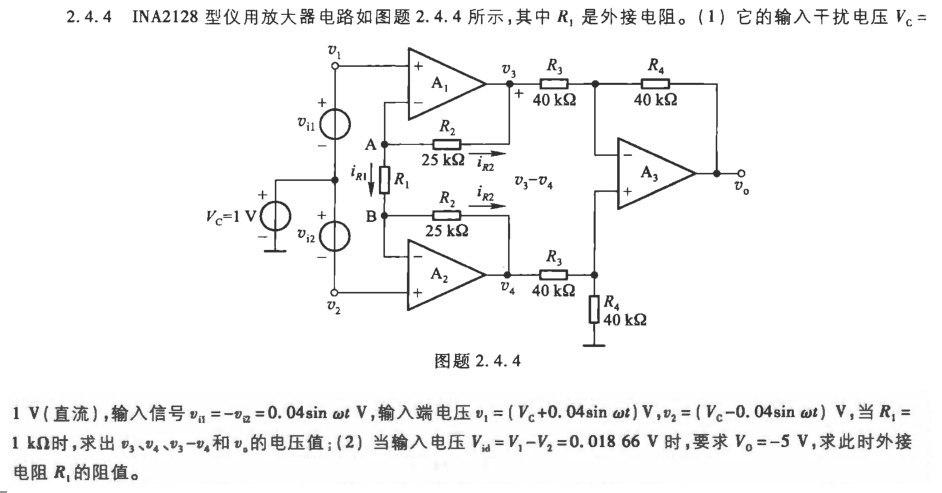
\includegraphics[width=\linewidth]{figures/Problem3-1}
  \label{fig:}
\end{figure}

\paragraph{Solution for Q1}

Since $A_1$ and $A_2$ are ideal operational amplifiers

\begin{equation*}
  \begin{aligned}
    v_A &= v_1 = V_C + v_{i1} \\
    v_B &= v_2 = V_C - v_{i2}
  \end{aligned}
\end{equation*}

Now we currents around $A_2$ can be calculated

\begin{equation*}
  \begin{aligned}
    i_{R2} = i_{R1} = \dfrac{v_A - v_B}{R_1} = \dfrac{v_{i1} + v_{i2}}{R_1} = 0.08 \sin \omega t \  \mathrm{mA}
  \end{aligned}
\end{equation*}



\begin{equation*}
  \begin{aligned}
    v_3 &= v_A + i_{R2} R_2 = \left( 1 + 2.04 \sin \omega t \right) \  \mathrm{V} \\
    v_4 &= v_B - i_{R2} R_2 = \left( 1 - 2.04 \sin \omega t \right) \  \mathrm{V}
  \end{aligned}
\end{equation*}



(I noted that the arrow below the first $R_2$ counted from top to bottom might be opposited)

We can then calculate the input voltage of $A_3$

\begin{equation*}
  \begin{aligned}
    V_{A3_{input}} = \dfrac{R_4}{R_3 + R_4} v_4  = \left( 0.5 - 1.02 \sin \omega t \right) \  \mathrm{V}
  \end{aligned}
\end{equation*}

For $R_4$, I assume the current direction is from left to right.

\begin{equation*}
  \begin{aligned}
    i_{R4} = \dfrac{v_3 - V_{A3_{input}}}{R_3} = \dfrac{0.5 + 3.06 \sin \omega t \  \mathrm{V}}{40 \  \mathrm{k\Omega}} 
  \end{aligned}
\end{equation*}

Finally

\begin{equation*}
  \begin{aligned}
    v_o = V_{A3_{input}} - i_{R_4} R_4 = - 4.08 \sin \omega t \  \mathrm{V}
  \end{aligned}
\end{equation*}

\paragraph{Solution for Q2}

Since $A_1$ and $A_2$ are ideal operational amplifiers

\begin{equation*}
  \begin{aligned}
    v_A &= v_1 = V_C + v_{i1} \\
    v_B &= v_2 = V_C - v_{i2}
  \end{aligned}
\end{equation*}

Now we currents around $A_2$ can be calculated

\begin{equation*}
  \begin{aligned}
    i_{R2} = i_{R1} = \dfrac{v_A - v_B}{R_1} = \dfrac{v_{i1} + v_{i2}}{R_1}
  \end{aligned}
\end{equation*}



\begin{equation*}
  \begin{aligned}
    v_3 &= v_A + i_{R2} R_2 = V_C + v_{i1} + \dfrac{v_{i1} + v_{i2}}{R_1} R_{2}\\
    v_4 &= v_B - i_{R2} R_2 = V_C - v_{i2} - \dfrac{v_{i1} + v_{i2}}{R_1} R_2
  \end{aligned}
\end{equation*}



(I noted that the arrow below the first $R_2$ counted from top to bottom might be opposited)

We can then calculate the input voltage of $A_3$

\begin{equation*}
  \begin{aligned}
    V_{A3_{input}} = \dfrac{R_4}{R_3 + R_4} v_4  = \dfrac{R_4}{R_3 + R_4} \left( V_C - v_{i2} - \dfrac{v_{i1} + v_{i2}}{R_1} R_2 \right)
  \end{aligned}
\end{equation*}

For $R_4$, I assume the current direction is from left to right.

\begin{equation*}
  \begin{aligned}
    i_{R4} = \dfrac{v_3 - V_{A3_{input}}}{R_3} = \dfrac{\left( V_C - v_{i2} - \dfrac{v_{i1} + v_{i2}}{R_1} R_2 \right) - \dfrac{R_4}{R_3 + R_4} \left( V_C - v_{i2} - \dfrac{v_{i1} + v_{i2}}{R_1} R_2 \right)}{R_3}
  \end{aligned}
\end{equation*}

Finally

\begin{equation*}
  \begin{aligned}
    v_o &= V_{A3_{input}} - i_{R_4} R_4 \\
    &= \dfrac{R_4}{R_3 + R_4} \left( V_C - v_{i2} - \dfrac{v_{i1} + v_{i2}}{R_1} R_2 \right \\
    &- \dfrac{\left( V_C - v_{i2} - \dfrac{v_{i1} + v_{i2}}{R_1} R_2 \right) - \dfrac{R_4}{R_3 + R_4} \left( V_C - v_{i2} - \dfrac{v_{i1} + v_{i2}}{R_1} R_2 \right)}{R_3} R_4
  \end{aligned}
\end{equation*}

When $V_1 - V_2 = v_{i1} + v_{i2} = 0.01866 \  \mathrm{V}$, $v_o = 5 \  \mathrm{V}$, we can solve for $R_1$

\begin{equation*}
  \begin{aligned}
    R_1 = 186 \  \Omega
  \end{aligned}
\end{equation*}





\end{document}